\documentclass[a4paper]{report}

\usepackage{graphicx}
\usepackage[utf8]{inputenc}

% Title Page
\title{Protokoll -  Network Sniffing und Portscanning}
\author{Manuel Neufeld, Dennis Tobias Rautenberg}


\begin{document}

\maketitle

\chapter{Intro}

\section{Versuchsaufbau}
Bei unserem Versuchsaufbau in unserem Labor wurde der bestehende Switch durch einen Hub ersetzt, um so alle Datenpakete aller Teilnehmer mitlesen/sniffen zu können.

\section{Software}
Wir verwenden für die uns bevorstehende Aufgabe das Betriebsystem Ubuntu und die Software Wireshark.

\begin{figure}[htb]
	\centering
		
\includegraphics[width=0.10\textwidth]{wireshark-logo.png}
	\caption{Wireshark Logo}
	\label{fig:wiresharklogo}
\end{figure}

\chapter{Grundlagen des Network-Sniffing}

\chapter{Aufgaben}

\section{a.) Analyse von typischem Netzwerkverkehr}

\subsection{Aufbauen einer TCP Verbindung}
Bauen Sie eine TCP Verbindung zu einem Dienst (z.B. http(s), ftp, smb, ssh, telnet) ihrer Wahl auf und beschreiben sie den Ablauf des Verbindungsaufbau/Verbindungsabbau (Sequenzdiagramm).

\begin{figure}[htb]
	\centering
		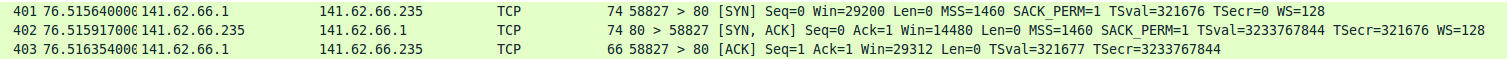
\includegraphics[width=1.25\textwidth]{laborergebnisse/screenshots/a_1.png}
	\caption{TCP Connection - HTTP Port: 80}
	\label{fig:tcpconnection}
\end{figure}

\iffalse HINT: schriftliche Beschreibung fehlt \fi


\subsection{Verbindungsversuch - geschlossener TCP Port}
Was passiert bei einem Verbindungsversuch auf einem geschlossenen TCP Port
(Sequenzdiagramm), z.B. telnet auf Port 161 (Befehl: telnet $<ip>$ 161).


\begin{figure}[htb]
	\centering
		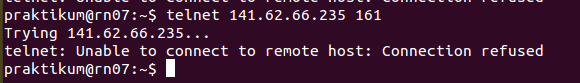
\includegraphics[width=1.25\textwidth]{laborergebnisse/screenshots/a_2-0.png}
	\caption{Verbindung per Telnet zu einem geschlossenen Port}
	\label{fig:tcpconnection}
\end{figure}

\begin{figure}[htb]
	\centering
		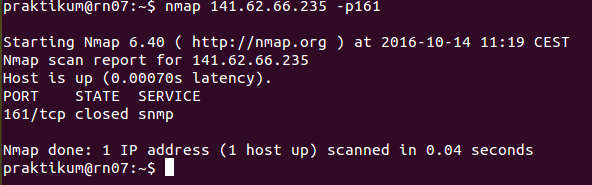
\includegraphics[width=1.25\textwidth]{laborergebnisse/screenshots/a_2-1.png}
	\caption{Nmap Port Scan - Closed Port}
	\label{fig:tcpconnection}
\end{figure}

\begin{figure}[htb]
	\centering
		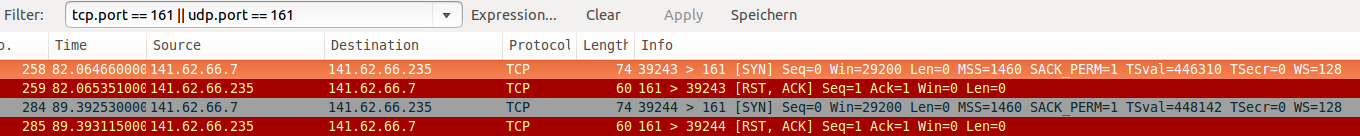
\includegraphics[width=1.25\textwidth]{laborergebnisse/screenshots/a_2-2.png}
	\caption{Capturing mit Wireshark}
	\label{fig:capturingwireshark1}
\end{figure}

Gescheiterter Verbindungsversuch aufgezeichnet mit Wireshark.

\newpage
\subsection{Beobachtung - DNS Traffic}
Sniffen Sie den DNS Traffic aus dem Netzwerkverkehr heraus, was beobachten Sie?

\begin{figure}[htb]
	\centering
		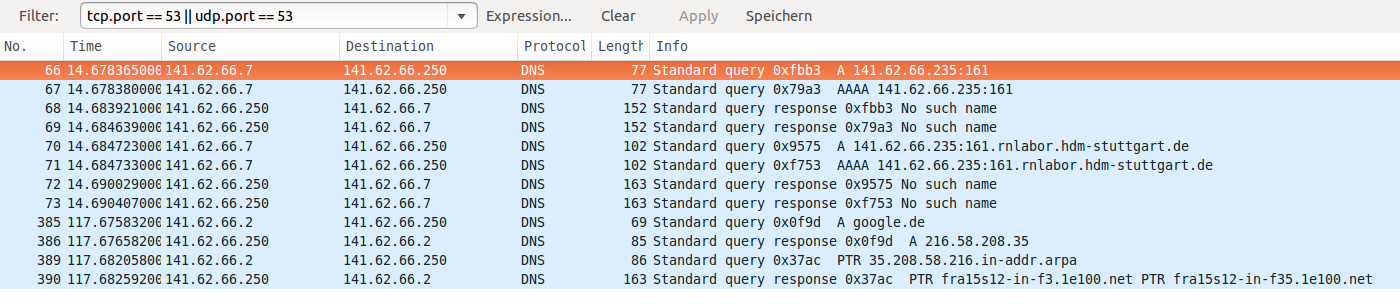
\includegraphics[width=1.25\textwidth]{laborergebnisse/screenshots/a_3.png}
	\caption{Capturing mit Wireshark}
	\label{fig:capturingwireshark1}
\end{figure}

\newpage
\subsection{Filtern von nicht IP basiertem Traffic}
Filtern Sie den nicht IP basierten Traffic heraus. Was bleibt nun noch übrig?

\begin{figure}[htb]
	\centering
		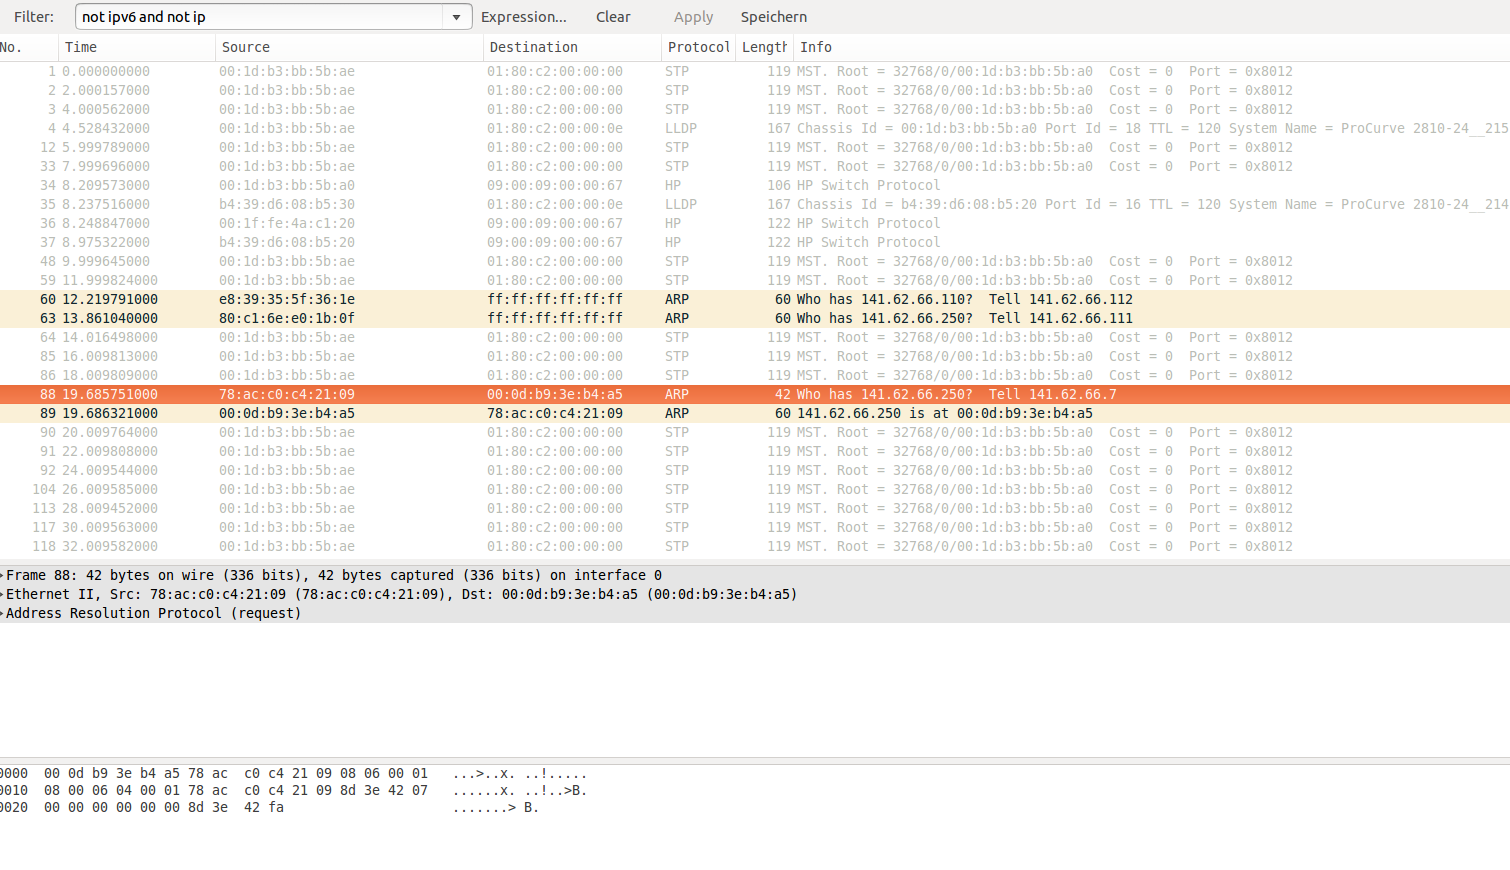
\includegraphics[width=1.25\textwidth]{laborergebnisse/screenshots/a_4.png}
	\caption{Capturing mit Wireshark}
	\label{fig:capturingwireshark1}
\end{figure}

\newpage

\section{b.) Sniffing von Passwörtern}
\subsection{Verbindung zu Telnet und FTP}
Verbinden Sie sich mit anderen Telnet und FTP Servern, nutzen Sie den PC Ihres Nachbarn!

\begin{figure}[htb]
	\centering
		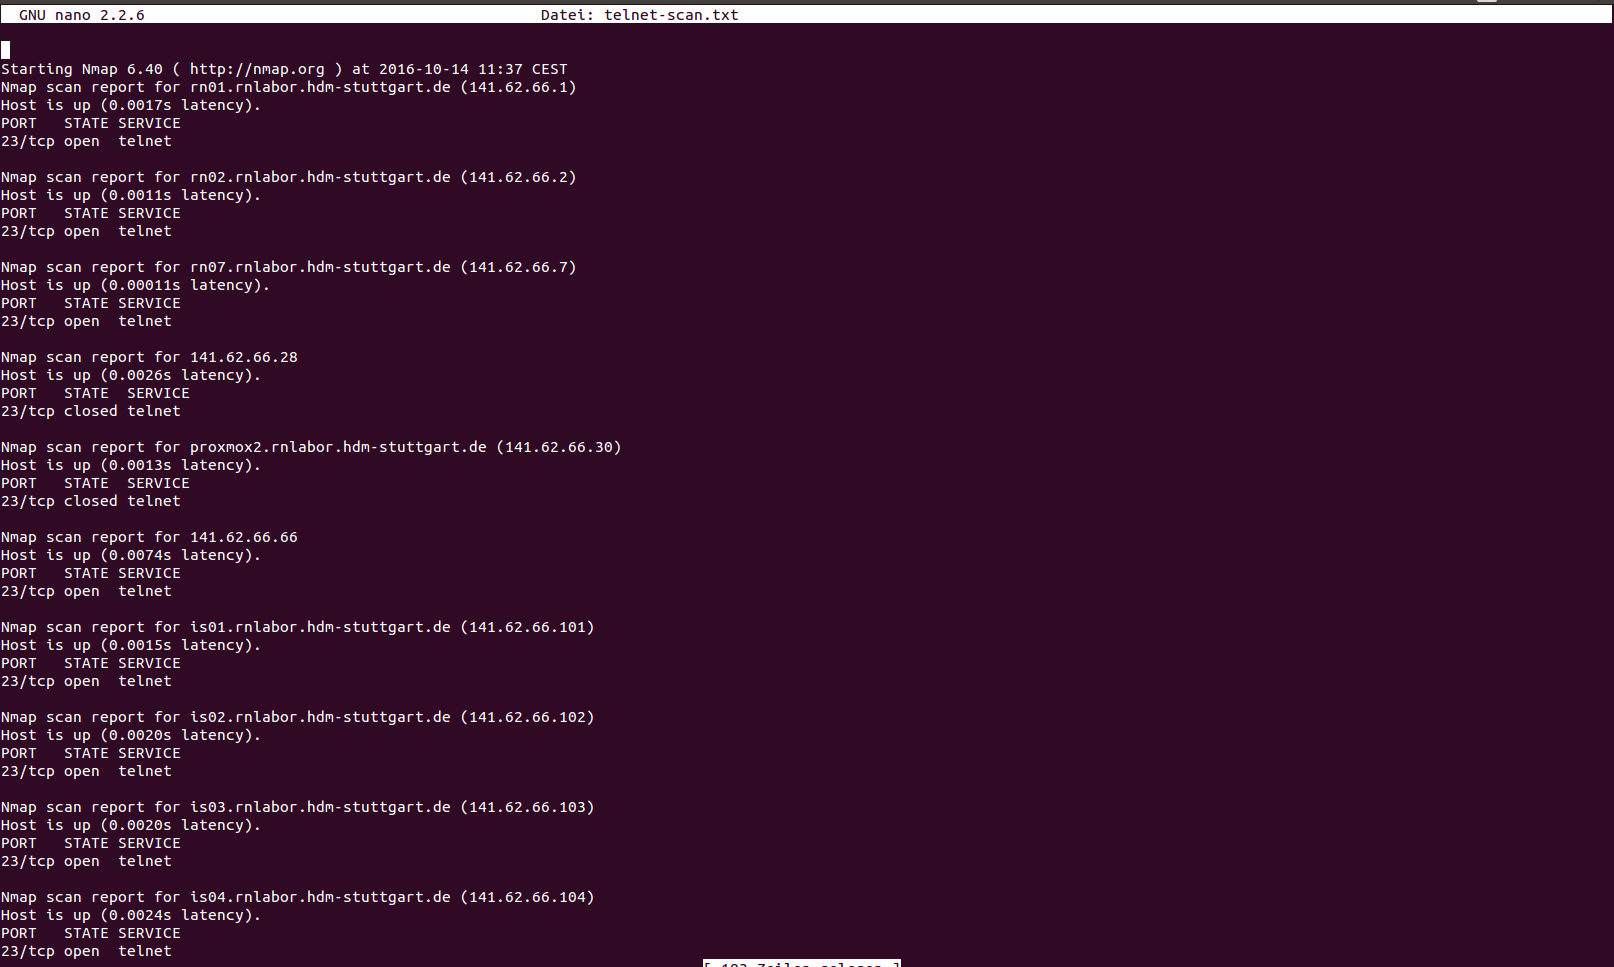
\includegraphics[width=1.25\textwidth]{laborergebnisse/screenshots/b_1.png}
	\caption{Capturing mit Wireshark}
	\label{fig:capturingwireshark1}
\end{figure}


\newpage
\subsection{Passwort Sniffing}
Versuchen Sie Passwörter und Benutzernamen anderer Benutzer, mitzusniffen. Filtern Sie gezielt die entsprechenden Pakete heraus.

\newpage
\subsection{Unterschied des übermittelten Passworts}
Beschreiben Sie den Unterschied zwischen dem FTP und Telnet Protokoll bezüglich der Passwort Übermittlung.

\section{c.) Portscanning / Nmap}
\subsection{Scannen vom Labornetz}
Scannen Sie das gesamte Labor Netz um aktive Systeme zu erkennen.
\subsection{Genauere Untersuchung eines Rechners}
Nehmen Sie einen Rechner genauer unter die Lupe und führen Sie einen detaillierten Portscan sowohl für TCP als auch für UDP Dienste durch.
\subsection{Verschiedene Scanverfahren}
Beobachten Sie die unterschiedlichen Scan-Varianten (Syn, Fin, Xmas, etc.) in Wireshark und analysieren Sie diese.

\chapter{Unterschied - Hub / Switch}

\section{Hub}
\begin{quote}
Ein Hub ist ein Kopplungselement, das mehrere Hosts in einem Netzwerk miteinander verbindet. In einem Ethernet-Netzwerk, das auf der Stern-Topologie basiert dient ein Hub als Verteiler fuer die Datenpakete. Hubs arbeiten auf der Bituebertragungsschicht (Schicht 1) des OSI-Schichtenmodells und sind damit auf die reine Verteilfunktion beschraenkt.
Ein Hub nimmt ein Datenpaket entgegen und sendet es an alle anderen Ports weiter. Das bedeutet, er broadcastet. Dadurch sind nicht nur alle Ports belegt, sondern auch alle Hosts. Sie bekommen alle Datenpakete zugeschickt, auch wenn sie nicht die Empfaenger sind. Fuer die Hosts bedeutet das auch, dass sie nur dann senden koennen, wenn der Hub gerade keine Datenpakete sendet. Sonst kommt es zu Kollisionen.\footnote{http://www.elektronik-kompendium.de/sites/net/1405161.htm} \end{quote}


\section{Switch}
\begin{quote}
Ein Switch ist ein Kopplungselement, das mehrere Hosts in einem Netzwerk miteinander verbindet. In einem Ethernet-Netzwerk, das auf der Stern-Topologie basiert dient ein Switch als Verteiler fuer die Datenpakete.
Die Funktion ist aehnlich einem Hub, mit dem Unterschied, das ein Switch direkte Verbindungen zwischen den angeschlossenen Geraeten schalten kann, sofern ihm die Ports der Datenpaket-Empfaenger bekannt sind. Wenn nicht, dann broadcastet der Switch die Datenpakete an alle Ports. Wenn die Antwortpakete von den Empfaengern zurueck kommen, dann merkt sich der Switch die MAC-Adressen der Datenpakete und den dazugehoerigen Port und sendet die Datenpakete dann nur noch dorthin.
Waehrend ein Hub die Bandbreite des Netzwerks limitiert, steht der Verbindung zwischen zwei Hosts, die volle Bandbreite der Ende-zu-Ende-Netzwerk-Verbindung zur Verfuegung.\footnote{http://www.elektronik-kompendium.de/sites/net/0811021.htm}
\end{quote}

\end{document}          
